\documentclass[conference]{IEEEtran}
\IEEEoverridecommandlockouts
% The preceding line is only needed to identify funding in the first footnote. If that is unneeded, please comment it out.

\usepackage{amsmath,amssymb,amsfonts}
\usepackage{algorithmic}
\usepackage{textcomp}
\usepackage{xcolor}
\usepackage{nicefrac}  % nicer inline fractions
\usepackage{tensor}  % allows fancy indices
\usepackage{siunitx}  % easy handling of value + unit (e.g. \SI{10}{\pF})
% \sisetup{}  % configure siunitx (e.g. locale = DE)
\sisetup{output-complex-root=\ensuremath{\mathrm{j}}, complex-root-position = before-number} % configures SI format 10 + j5 for complex numbers (instead of 10 + 5i)

\usepackage{listings}  % code listings
\usepackage{enumerate}
\usepackage{booktabs}  % nicer tables (e.g. \toprule)
\usepackage{verbatim}  % inline code (\verb||)
\usepackage[european, siunitx, RPvoltages]{circuitikz}  % draw circuit diagrams
\usepackage{enumitem}
\setlist[itemize]{label=\rule[0.5ex]{0.6ex}{0.6ex}} % black squares for itemize
\usepackage{flushend}

\usepackage{graphicx}
\graphicspath{{./figures/}}

\usepackage{csquotes} % removes biber warning
\usepackage[  % ieee style citations (e.g. [1])
	backend     = biber,
	maxbibnames = 99,
	autocite    = footnote,
	style	    = ieee,
	citestyle   = numeric-comp,
	doi=false, isbn=false
]{biblatex}
\addbibresource{bibliography/bibliography.bib}

\usepackage[nobiblatex]{xurl}  % line breaks in URLs
% last imports
\usepackage[bookmarksopen,colorlinks,citecolor=black,linkcolor=black, urlcolor = black]{hyperref}

% after hyperref! 
\usepackage[noabbrev, nameinlink]{cleveref} 
% e.g. \cref{label} or \Cref(label) for capital letter
% configure cleveref not to use brackets around equation references
\creflabelformat{equation}{#2\textup{#1}#3} % Equation references without parentheses

% add missing hyphenations
\hyphenation{im-ple-men-ta-tions}

\def\BibTeX{{\rm B\kern-.05em{\sc i\kern-.025em b}\kern-.08em
    T\kern-.1667em\lower.7ex\hbox{E}\kern-.125emX}}

\begin{document}

\title{Energy-Efficient SRAM Cells for Near-Threshold Computing\\
{\normalsize 354.072 Seminar Mixed-Signal ICs, Summer Term 2021}
\thanks{Draft submitted \today.}
}

\author{\IEEEauthorblockN{Severin Jäger}
\IEEEauthorblockA{
	M.Nr. 01613004 \\
	severin.jaeger@tuwien.ac.at}
}

\maketitle

\begin{abstract}
Operation at voltages near the transistor threshold allows for computation at minimal energies. However, predominant memory technologies operate poorly in those conditions. To mitigate this bottleneck, several alternative cell designs and technological improvements were proposed in the literature. This seminar thesis discusses selected publication from this field to investigate the design space for near-threshold SRAM cells as there is not dominant solution yet.
\end{abstract}

\section{Introduction} \label{sec:intro}

Modern embedded systems require energy-efficient processors. One promising approach is near-threshold computing, where supply voltages are decreased towards the transistor threshold voltage. This reduces the achievable clock frequencies but increases the energy efficiency far beyond this reduction. However, the static random access memory (SRAM) cells used in the caches of modern embedded processors are a critical component for this technique as established memory cells do not operate reliably at low voltages \cite{De2017}. In particular, the standard six transistor SRAM cell suffers from process variations, soft errors caused by external radiation and noise in near-threshold operating conditions.

As caches make up a significant share of the die size of systems-on-a-chip (SoCs), the reduction of voltage and thus energy consumption of this circuitry is of high importance. However, alternative approaches both on the technology and the memory cell level are required to achieve reliable near-threshold SRAM. In particular, SRAM cells are increasingly sensitive to radiation-induced bit-flips as voltages are reduced, lack sufficient read stability in larger memory arrays, or do not exploit the advantages coming with lower voltages sufficiently. Once these challenges are tackled, near-threshold computing might enable extremely efficient embedded systems for instance in medical implants or extreme edge computing.

This seminar thesis investigates recent contributions tackling some of the aforementioned limitations of standard SRAM cells in near-threshold setups. The rest of this work is structured as follows. Section~\ref{sec:background} presents basic concepts of near-threshold computing and SRAM cells. In the following, Sections~\ref{sec:paper1} to \ref{sec:paper3} discuss three recent publications investigating problems with SRAM cells in the context of voltage scaling. Finally, major outcomes are summarised in Section~\ref{sec:conclusion}.

\section{Background} \label{sec:background}

\subsection{Near-Threshold Computing} \label{sec:background:ntc}

During the last two decades the so-called Dennard scaling that basically stated that increasing transistor counts come at constant power consumption has come to an end. Modern high-performance chips are frequently limited by their power consumption \cite{Pinckney2017}. Thus, the so-called dark silicon era \cite{De2017} has started. This means that not all functional units of a chip can be active at the same time to keep the power consumption inside the thermal limits.

In general, the power consumption of a digital integrated circuit can be estimated as \cite{Flynn2011}

\begin{equation*}
	P_{total} = \frac{CV^2f}{2} + I_{leak} V
\end{equation*}

with the device capacitance $C$, the supply voltage $V$ the switching frequency $f$ and the leakage current $I_{leak}$. The first component is called dynamic power as it depends on the clock frequency and the latter static power.

In order to reduce the power consumption, the voltage can be reduced. However, this affects the gate delay as \cite{Pinckney2017}

\begin{equation*}
	d_{gate} \propto \frac{1}{f} \propto \frac{V}{(V-V_{th})^\alpha}
\end{equation*}

with the transistor threshold voltage $V_{th}$ and the modelling parameter $\alpha > 1$. So if the supply voltage is reduced, the circuit becomes slower. While the dynamic power decreases significantly, the static power plays an increasing role. This is due to the fact that the leakage current increases as the threshold voltage is reduced together with the supply voltage to maximise the operating frequency.

Several techniques like dynamic voltage and frequency scaling (DVFS), clock gating, and power gating have emerged to find a suitable trade-off between performance and energy consumption. One rather radical approach is near-threshold computing, i.e. reducing the supply voltage to the proximity of the transistor threshold voltage. This is desirable as it allows for the optimum energy per operation. The so-called minimum energy point (MEP) is usually slightly above the threshold and depends on process variations and the runtime conditions \cite{Golanbari2020}. At lower voltages, the achievable clock frequency drops drastically and increased leakage currents dominate while voltages above the MEP are dominated by dynamic power.

Still, near-threshold computing comes with several design challenges. Firstly, the clock frequency of such a chip is reduced by a factor of $50$ to $100$ \cite{Dreslinski2010}. To utilise this, significant changes in the architecture of the SoC are required. Usually, several parallel execution units are operated simultaneously. This is possible as several parallel cores can operate within the thermal limits of the chip \cite{Pinckney2017}. Furthermore, cell libraries have to be adapted for near-threshold operation \cite{De2017}. Suitable libraries have however already been developed \cite{Zhou2012}.

The near-threshold computing community aims at maximising the operations per watt of power consumption. Recent designs like the PULP platform \cite{Rossi2017} target at ultra-low power sensor nodes with notable processing requirements. Such throughput-oriented applications are one promising application field for near-threshold computing, however \cite{Dreslinski2010} sees significant potential for this technology in servers and even in personal computing.

\subsection{Static RAM} \label{sec:background:sram}

Typically, static memory is organised in arrays. Each memory cell holds one bit and is connected both to a row address (frequently called word line) and a column address (frequently called bit line). Given a memory address, the row is selected with a decoder. To avoid interference with the non-accessed cells, memory cells have to be in a high-impedance state when they are not selected. In each column, a read-write-amplifier reads or writes the bit lines to or from an output register that allows for fast word-wise read and write operations~\cite{Tietze2019}.

% 6T cell
The predominant SRAM cell is composed of six transistors and thus called 6T cell. It is depicted in \Cref{fig:6t} and consists of two cross-coupled inverters (transistors $M_1$ to $M_4$) storing one bit of information and the access transistors $M_5$ and $M_6$ ensuring the high-impedance state. The cell is constructed differentially, i.e. the voltage at node $\bar Q$ is the inverse of the voltage at node $Q$. In case a logic $1$ is stored, the voltage at node $Q$ is almost $V_{DD}$ while the voltage at $\bar Q$ is almost $0$. There are two differential bit lines, this reduces disturbances~\cite{Tietze2019}.

\begin{figure}
	\centering
	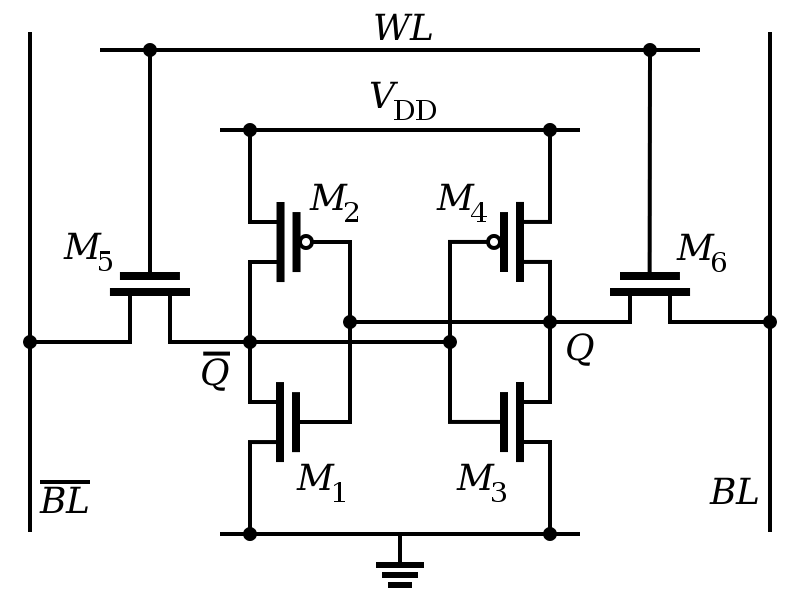
\includegraphics[width=6.5cm]{6t_cell.png}
	\caption{Standard 6T SRAM cell \cite{6t}}
	\label{fig:6t}
\end{figure}

% read
In order to read the information stored in a cell the word line is set high. Both bit-lines are pre-charged to $V_{DD}$. As one of the nodes $Q$ and $\bar Q$ is pulled to $V_{DD}$ and the other one to ground, one of the access transistors (the one on the side pulled to ground) will be conducting, while the other one remains in a non-conducting mode. Assuming the cell stores a $0$, $M_3$ is pulling $Q$ to ground while $M_6$ is pulling it to $V_{DD}$. Therefore it is required that $M_3$ is stronger in the sense that it pulls the whole bit line to ground \cite{Senousy2016}.

% write
The write operation requires the word line to be set high, too. Simultaneously, the write amplifier drives both the bit line and the inverted bit line. Again, the node $Q$ or $\bar Q$ is driven both from the cross-coupled inverters and the bit line. This is resolved by the requirement that the access transistors are stronger than the pull-up transistors \cite{Senousy2016}.

% 6T near threshold, supply voltage dependency
So the relative dimensions of the pull-up, pull-down and access transistors have to be well-balanced to allow for suitable read and write performance in standard operating conditions. However, as the noise margins of the 6T cell (read static noise margin (SNM) and write noise margin (WNM)) decrease with the supply voltage \cite{Senousy2016} and process variations that reduce those margins play an increasing role at near-threshold voltages \cite{Dreslinski2010}, this cell is hardly applicable for reliable operation at near-threshold voltages. 

% Challenges and potential solutions
Dreslinski et al. \cite{Dreslinski2010} propose three conceivable ways to overcome this limitations: Alternative SRAM cell designs, robustness analysis in combination with optimisation of the 6T cell and higher-level cache architecture measures. While the latter will not solve the physical limitations of near-threshold SRAM, several transistor and technology level implementations exist in the literature for the earlier approaches.

\begin{figure}
	\centering
	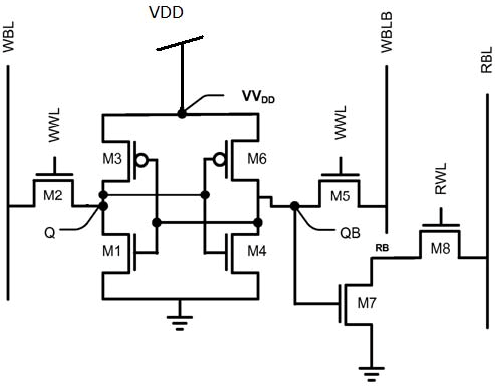
\includegraphics[width=7.5cm]{8t_cell.png}
	\caption{Standard 8T SRAM cell \cite{8t}}
	\label{fig:8t}
\end{figure}

% Standard 8T cell
One well-established alternative cell design is the standard 8T cell proposed in \cite{Chang2008}. It is depicted in \Cref{fig:8t} and decouples the read path from the write path with the additional transistors $M7$ and $M8$. Thus, it introduces read stability, i.e. a read operation cannot flip the stored data \cite{Cho2020}. Additionally, in a near-threshold scenario the 8T cell features higher noise margins than the 6T cell and a reduced error rate \cite{Gebregiorgis2019}.

On the other hand the 8T cell comes with additional complexity. Firstly, an additional bit line (RBL) and an additional word line (RWL) are required. Furthermore, the additional transistors obviously increase the cell area and thus decrease the memory density. However, the required optimisations for near-threshold operations increase the size of the 6T cell as well, thus this effect becomes less significant with decreased voltages \cite{Dreslinski2010}.

\section{10T SRAM Cells for Large Memory Arrays} \label{sec:paper1}

In \cite{Gupta2019}, three application-specific SRAM cells composed of ten transistors (10T) are proposed. The authors address the limitations of the standard 8T SRAM cell when operated in long arrays (i.e. many words in one block of memory) in a near-threshold configuration.

In particular, the $I_{ON}/I_{OFF}$ ratio of this cell is insufficient for arrays in the magnitude of $1024$ cells per read bit line. So the leakage current of the $1023$ non-selected cells might be large enough to alter the voltage level on the read bit line in a way that the read amplifier reads the wrong value. Another issue with the 8T cell is the fact that the leakage current depends on the stored data bits. \Cref{fig:leakage} visualises these problems. As a result, topologies consisting of local read bit lines connecting eight SRAM cells which are connected with further circuitry to a global read bit line are used. This additional complexity comes with a significant area overhead.

\begin{figure}
	\centering
	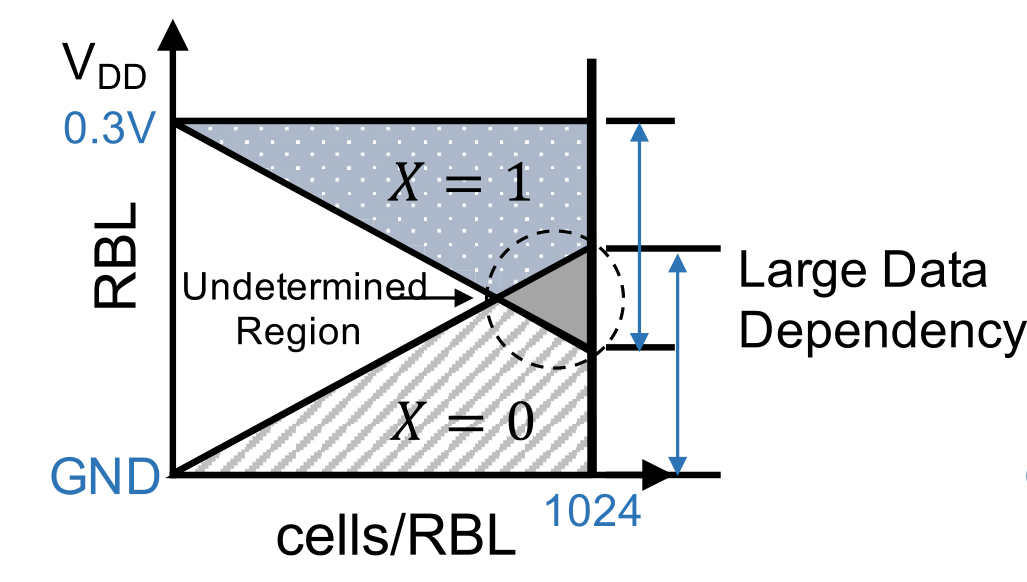
\includegraphics[width=6cm]{leakage.png}
	\caption{Reduced effective read bit-line swing in large arrays \cite{Gupta2019}. Once the undetermined region is reached, the memory will not operate reliably even without noise.}
	\label{fig:leakage}
\end{figure}

% Proposed cells
The authors refer to some alternative cell designs \cite{Calhoun2007, Kim2008, Pasandi2015} but outline their shortcomings regarding area, data-dependent performance and energy consumption. Thus, they propose the three SRAM cells depicted in \Cref{fig:gupta}. All three are designed for an improved $I_{ON}/I_{OFF}$ ratio by reducing leakage currents. Thus, they reuse the cross-coupled inverters and the write access transistors from the 8T cell and feature modified read ports. From an array perspective they are except for the 10T-P3 cell which requires an inverted read bit line interchangeable with the 8T cell as they need two words lines (read and write), differential write bit lines, and a single read bit line.

% details
While the 10T-P1 cell is aimed at high performance it still suffers from a data-dependent leakage. In contrast, the 10T-P2 and the 10T-P3 are designed for low power and low area respectively and show a widely data-independent leakage current. In combination with the relative to the 8T cell drastically reduced $I_{OFF}$, they are eligible for long read bit lines.

\begin{figure}
	\centering
	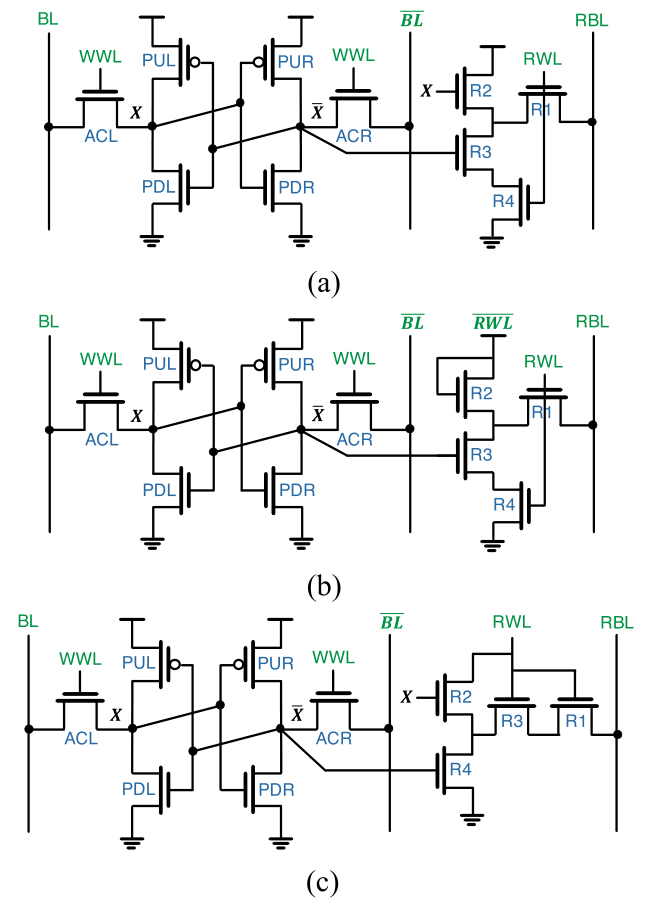
\includegraphics[width=8.5cm]{cells_gupta.png}
	\caption{SRAM cells 10T-P1\,(a), 10T-P3\,(b), and 10T-P2\,(c) proposed in \cite{Gupta2019}}
	\label{fig:gupta}
\end{figure}

% evaluation technology and method
To evaluate the proposed cell designs, the authors implemented a \SI{128}{kB} array consisting of four blocks with $1024$ words of \SI{32}{bits} each in a \SI{32}{nm} process. This was done for all three proposed cells as well as for the reference designs introduced in \cite{Calhoun2007, Kim2008, Pasandi2015}. The following design details were crucial for the performance of the cells: In the 10T-P1 cell, the read transistor $R3$ was designed $1.67$ times wider than in all other designs trading off the additional read performance of this cell topology with increased standby power consumption. Furthermore, the inverted read word line had to be provided to the 10T-P3 cell. To minimise the overhead, this signal was shared between two rows. This however leads to half-selected cells that contribute to the overall power consumption.

All designs were simulated and the following results were achieved.

\subsubsection{Area}
All three proposed cells do in contrast to the cells proposed in \cite{Calhoun2007, Kim2008, Pasandi2015} not require any PMOS transistors outside the cross-coupled inverters. This reduces the size of the n-well and leads to narrower cells. This reduces the bit line lengths. Consequently, the dynamic read performance is improved and the dynamic power consumption is reduced. Despite all three proposed cells being smaller than the reference ones, the 10T-P3 cell is clearly the most compact design.

\subsubsection{Read Bit-Line Swing}
The read bit-line swing is quantified as a fraction of the difference between $V_{DD}$ and ground. The simulation shows that the 10T-P1 cell outperforms previous designs, but shows a data dependent bit-line swing. In contrast, the T10-P2 and T10-P3 cells do not show notable data dependencies, however the earlier outperforms all other evaluated cells clearly as it reaches almost \SI{100}{\%} in most evaluated scenarios. This indicates a minimal leakage current.

\subsubsection{Standby Leakage Power}
Regarding the consumed power while holding the data, all proposed cells outperform the reference cells in the near-threshold region. However this metric itself is insufficient, as SRAM is used in caches and thus frequently accessed.

\subsubsection{Energy per Access}
The authors evaluated the energy consumed by one read access as a function of supply voltage and activity factor (i.e. the fraction of clock cycles in which the SRAM is accessed). They observed that the minimum energy point lies in the near-threshold area for high activity factor and is shifted to slightly higher voltages as the activity is reduced. The 10T-P2 cell outperforms the other cells for all investigated activity factors.

To sum up, the authors have presented three rather specific SRAM cells that are designed with applications in large arrays in mind. One cell has an excellent minimal access voltage, another one features a very low energy per access and a third cell shows a small footprint. All cells outperform previous designs. Still, there is no cell unifying the advantages of all three cells available, thus a careful cell selection depending on the application is unavoidable.

\section{One-Sided Schmitt-Trigger-Based 9T SRAM Cell} \label{sec:paper2}

In a near-threshold setup, the charge held by one SRAM cell is significantly smaller than in regular super-threshold operation. Thus, the probability of bit-flips induced by alpha particles or high-energy radiation is higher and measures against these so-called soft errors are of great importance. Error-correcting codes (ECC) are a well-established technique to mitigate soft errors in the memory system. However, it requires additional hardware and thus area. A common trade-off is that the ECC hardware is able to correct one bit per word \cite{Nayak2018}.

As the bit-error probability is relatively high in a near-threshold regime and as the memory cells are very small, it is likely that two or more neighbouring SRAM cells are affected by one soft error. Frequently, bit-interleaving is used to avoid multi-bit errors that cannot be resolved by simple ECCs. In a bit-interleaving configuration, words within one row are not stored sequentially but interleaved in the sense that firstly the bits with index $0$ of all words are stored then the ones with index $1$ and so on \cite{Nayak2018}. This drastically reduces the probability of multi-bit errors within a word. However, this requires that multiple word are stored in one row. As all of them are connected to the same word select signal and simultaneous read and write operations within one row are desirable, read operations overlapping with write operations in the same row might be disturbed \cite{Cho2020}. Common SRAM cells like the 8T cell require some form of write-back mechanism that consumes area and energy to resolve this issue.

Thus, Cho et al. \cite{Cho2020} evaluated existing cell designs that do not require such a write-back and found that they either use a differential bit line for read and write and consume significant area and energy or are rather complicated and hence have a large die footprint. Therefore, they propose a novel nine-transistor cell that is depicted in \Cref{fig:cho}. It is based on an inverter ($PUL1$, $PDL2$) with gating transistors ($PUL2$, $PDL1$) cross-coupled with a Schmitt Trigger inverter ($PUR$, $PDR1$, $PDR2$, $NF$). Similarly to the 6T cell, he information itself is stored in the nodes $Q$ and $QB$. Additionally, the access transistor $PG$ connects the memory cell to the single bit line. Additionally, the cell is connected to a row-based word line signal and two column-based word line write signals WWLA and WWLB.

\begin{figure}
	\centering
	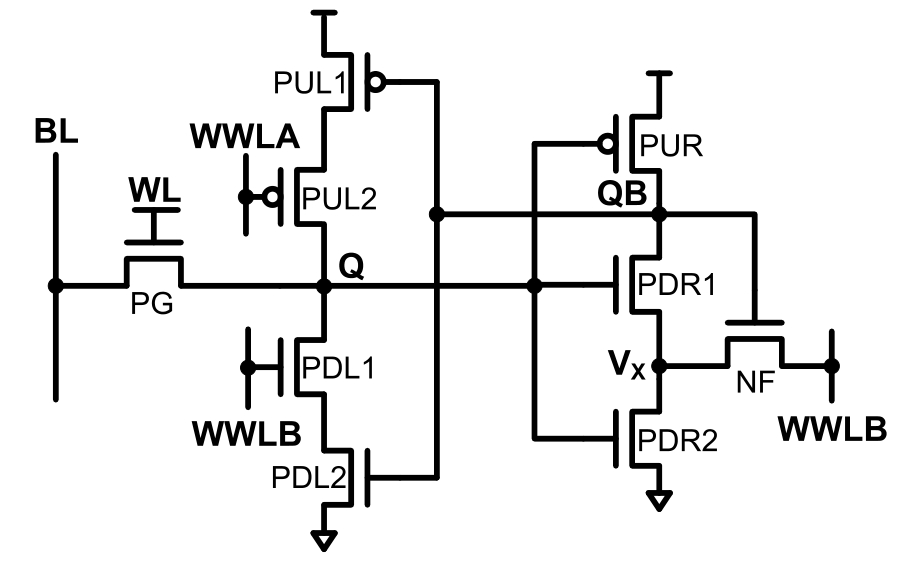
\includegraphics[width=7.5cm]{cell_cho.png}
	\caption{9T SRAM cell proposed in \cite{Cho2020}}
	\label{fig:cho}
\end{figure}

% read
In order to read the value stored in a cell, the word line signal has to be set while the WWLA signal is set to $0$ and the WWLB signal is set to $1$. This ensures that the left inverter drives the $Q$ node and that this voltage is propagated to the bit line via the $PG$ transistor. One major advantage of the Schmitt Trigger based approach is the higher robustness against disturbances coming from the bit line. Due to the hysteresis of the Schmitt Trigger, the static read noise margin is significantly increased relative to cells based on two standard CMOS inverters or even two Schmitt Trigger inverters.

% write
The Schmitt Trigger based cell comes at the price of increased write complexity. The write process differs between writing $0$ and writing $1$. In the former case, the signals WL and WWLB are set. After the $0$ is driven to the bit line, the WWLA signal is set for a relatively short time to power gate node $Q$ and flip the Schmitt Trigger inverter. In case a $1$ is written, WL is set and WWLA remains $0$. After the write driver has set the bit line to $1$, WWLB is set to $0$ for a short time. This disconnects $Q$ from the ground. During this time, the feedback mechanism of the Schmitt Trigger is removed, thus the increased robustness against write processes is not given. Still, the write-$1$ ability is insufficient. Thus, the WWLB signal is not only driven to $0$ but even to a slightly negative voltage. This reduces the trip voltage of the Schmitt Trigger and simplifies write operations.

% half select
One major drawback of this cell is the presence of half-select issues when the cell is operated in a bit-interleaving fashion as it is not read-disturbance free. Due to the good read stability of the cell, there are no major problems with row half-selected cells (connected to the same WL), but this is not the case for column half-selected signals (connected to the same WWLA and WWLB). As the transistors $PUL2$ and $PDL1$ power gate the $Q$ node, the half-selected cells can be floating while the selected cells are written. As WWLA and WWLB are toggled only for a short period, the capacitance of node $Q$ is large enough to maintain the stored value.

% evaluation
To evaluate the design, the proposed cell and some alternative approaches were drawn in a \SI{22}{nm} FinFET process and simulated with a Monte Carlo method. The following results were achieved.

\subsubsection{Area} The proposed cell is \SI{24}{\%} larger than the standard 8T cell, but still significantly smaller than comparable near-threshold cells without the necessity for write-back.

\subsubsection{Read Stability} The Schmitt Trigger based 9T cell is not read-disturbance free, yet it outperforms other cells without read-disturbances. Thus, it can be operated at lower voltages without losing sufficient read stability than comparable designs.

\subsubsection{Energy per Operation} One major advantage of the proposed cell is its low read energy consumption due to its single-ended bit line. Here it outperforms the reference designs. In contrast, it has a relatively high write energy consumption. However, as read accesses dominate in caches, its overall energy per operation in a realistic setting is competitive.

\subsubsection{Energy-Delay-Product} At the optimal voltage, the proposed cell has a higher energy-delay-product than the other evaluated cells. This makes it extremely efficient for near-threshold computing.

Overall, the one-sided Schmitt Trigger 9T cell is compact and energy-efficient and features a high static read noise margin. On the other hand, it is not read-disturbance free and requires a relatively complex select logic with very specific timing constraints. Still, it is applicable for bit interleaving without write-back and thus for reliable near-threshold SRAM blocks.

\section{Near-Threshold Operation of 8T FinFET SRAM Cells} \label{sec:paper3}

During the last years, FinFET transistors have gained significant prevalence in digital integrated circuits. They resolve the scaling issues regarding standby power and device variability of bulk-CMOS devices by offering better control over the channel and the option to bias front and back gates independently. However, they tend to consume more area than bulk devices at a comparable technology node.

FinFETs are a particularly promising technology for SRAM cells as leakage power plays a notable role in memory power consumption. Furthermore, they allow for reduced delay as the $I_{ON}$ current increases. Overall, their $I_{ON}/I_{OFF}$ ratio is significantly increased as compared to bulk-CMOS cells. As discussed in Section~\ref{sec:paper1}, this enables high read static noise margins and long memory columns. Besides the aforementioned area overhead, FinFET SRAM potentially faces data stability issues due to the discrete fin number, however this is not treated further in this work.

Turi and Delgado-Frias \cite{Turi2017} are the first ones to evaluate the potential of FinFETs for 8T SRAM cells both in full-$V_{DD}$ and near-threshold conditions. They compare different biasing strategies for the transistors and seek for optimal configurations. They mainly focus on the option of biasing the FinFET back gates. In particular they distinguish two operation modes:

\begin{itemize}
	\item Shorted gate (SG): In this configuration, back and front gates are shorted and there is only one gate terminal. This corresponds to the typical operation mode of bulk-CMOS transistors.
	\item Low power (LP): Here, the front and back gates are independent terminals. This is used to reverse-bias the back gate\footnote{For n-type transistors a negative voltage (e.g. \SI{-0.2}{V}) is used, in the case of p-type devices a voltage larger than $V_{DD}$ (e.g. $V_{DD} + \SI{0.2}{V}$) is applied.} to reduce the leakage current significantly while simultaneously reducing the on-current. However, it requires additional voltage generation circuitry and wiring.
\end{itemize}

As the paper focusses on the 8T cell, the authors figured out eight different configuration combinations as they mapped different transistors to those operation modes. The read port (transistors $M7$ and $M8$ in Figure~\ref{fig:8t}) is implemented in the SG mode in all combinations to maintain fast read operations while the following transistor pairs are evaluated in all different combinations of SG and LP:
\begin{itemize}
	\item Access transistors ($M2$ and $M5$),
	\item N-type inverter transistors ($M1$ and $M4$),
	\item P-type inverter transistors ($M3$ and $M6$).
\end{itemize}

For evaluation, two 6T cells (all transistors LP and all transistors SG) and the manifold of 8T variants were implemented in a silicon-on-insulator process with \SI{30}{nm} gate length. The memory array for evaluation is as in \cite{Gupta2019} $1024$ words of $32$ bits large. All analyses were conducted in a Spice-based simulation environment.

Firstly, the different cell designs were evaluated at full $V_{DD}$, i.e. \SI{1}{V}. It was observed that almost all 8T variants outperformed the 6T cells in terms of the energy-delay-product (EDP). In general, the authors concluded that the 8T cell allows for easier configuration for good performance than the 6T cell which has to trade-off read and write performance. Furthermore, the LP configuration with reverse biasing drastically decreased leakage currents both in 6T and 8T designs (by up to \SI{97}{\%}). Interestingly, the best energy-delay-product at this voltage was achieved by the LP\_INV cell which uses reverse-biasing (LP) in both the n-type and p-type inverter transistors but SG in the access transistors. It has \SI{74}{\%} less EDP than the 6T cell in SG configuration.

When it comes to near-threshold operation around the minimum-energy point (at \SI{0.6}{V}), the 6T LP cell has a higher energy-delay-product than the SG variant as the read delay of the latter skyrockets already above the threshold voltage. Still, both 6T designs operate with higher energy-efficiency than at full $V_{DD}$. The 8T cells in contrast show a less steep increase in delay and thus profit from voltage scaling even more. Again, the LP\_INV cell achieves the best EDP of \SI{9}{ps \cdot fJ}, this corresponds to a \SI{65}{\%} decrease as compared to full-$V_{DD}$ operation and a \SI{84}{\%} reduction relative to the best 6T design in the near-threshold regime. The leakage current hardly differs between 6T and 8T cells, however LP designs perform more than one magnitude better than SG cells. In general, the leakage current decreases linearly with the supply voltage. When it comes to noise margins, a decrease is observed with reduced supply voltages. Again, the LP 8T cells show the highest margins in the near-threshold regime. The only performance demerit of the LP designs is the reduced write speed. However, as discussed in Section~\ref{sec:paper2}, read accesses dominate in cache applications. Thus, this does hardly limit the potential of this technology.

In the last sections, the authors investigated the performance of the studied FinFET SRAM designs in different memory arrays, unter parameter and voltage variations, and in different temperatures. This however goes beyond the scope of this seminar thesis.

In conclusion, the authors have shown the potential of FinFETs for SRAM cells in near-threshold applications. Mainly, they outlined the advantages of both the 8T cell and the low-power configuration with reverse back-gate biasing. Specifically, they pointed out that the LP\_INV cell with reverse-biased back-gates in the inverter transistors is a promising candidate for energy-efficient SRAM as it has a minimal leakage current, excellent static noise margins, and an unbeaten energy-delay-product both in the full-$V_{DD}$ and in the near-threshold operation. Thus, FinFETs might offer reliable near-threshold SRAM. However, throughout the publication the area of the proposed cells was not elaborated on. Thus, it remains unclear whether FinFET-based SRAM can compete with bulk-CMOS memory when it comes to integration density.

\section{Conclusion} \label{sec:conclusion}

This seminar thesis discussed the challenges for SRAM design in near-threshold computing. As the well-studied 6T cell delivers insufficient performance at these voltages, there is room for alternative solutions. The standard 8T cell is one promising candidate, however it might have a too high leakage current for large arrays or cause write-back overhead in bit-interleaving scenarios. These issues were discussed in the publications discussed in Sections~\ref{sec:paper1} and \ref{sec:paper2}, which proposed SRAM cells partially mitigating these shortcomings. As none of the discussed cells solves all relevant challenges in near-threshold SRAM design, it is likely that there will be further progress in this field in the near future. Another conceivable development is that technological advances like FinFETs will allow sufficient performance of existing cell designs like the 8T cell as discussed in Section~\ref{sec:paper3}.

As near-threshold computing is still an emerging field, there are several developments ongoing and the satisfying industry standard for SRAM in this context has not established yet. Thus, cell selection will remain an application-specific trade-off in the near future as several interesting designs including the ones presented in this thesis with their strengths and weaknesses were proposed by academia in the last years.

\listoffigures

\printbibliography

\end{document}
